% Target: 3-4 blz

In this section, the generic algorithm is explained. First, we cover some of the constraints we made for the algorithm. Second, we give the algorithm itself which is then, finally, explained in more detail in the following subsections.

%\begin{figure}[h]
%    \centering
%    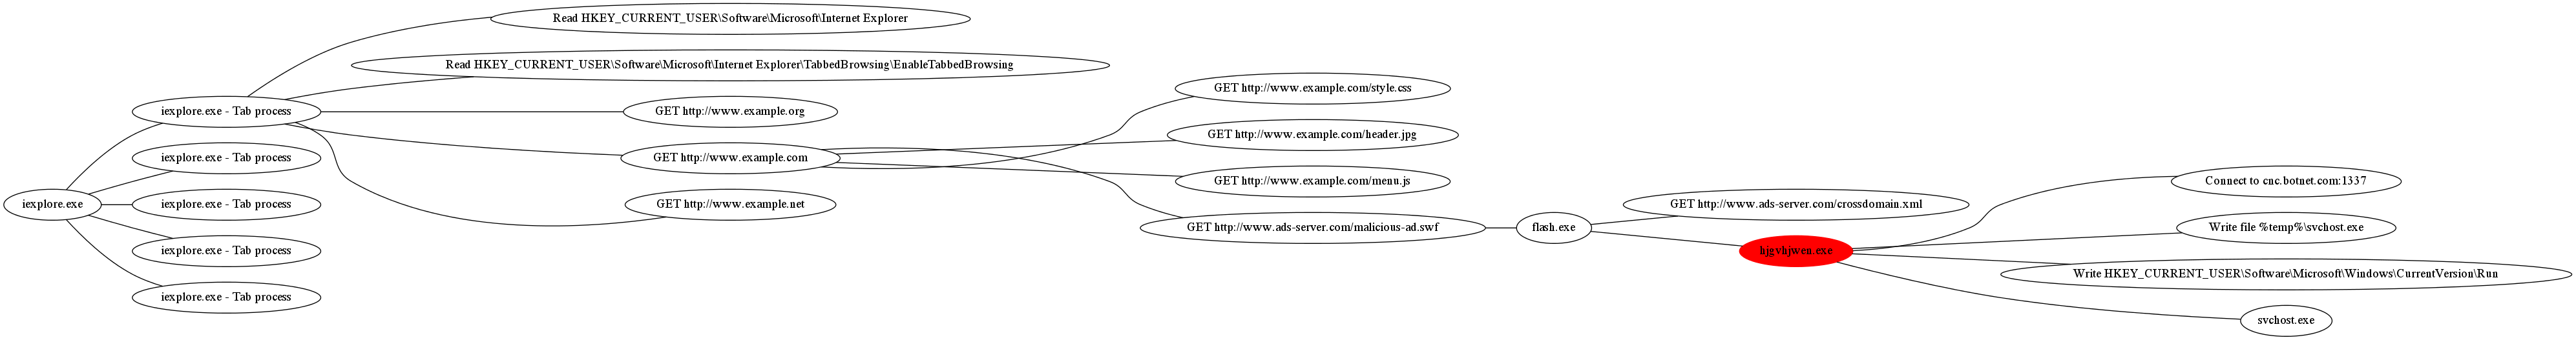
\includegraphics[width=17cm]{Images/alg_tree.png}
%    \caption{An example of the graph}
%    \label{fig:alg_tree}
%\end{figure}

\subsubsection{Design considerations}

One of the major considerations that was made, is the fact that the algorithm should work on multiple operating systems and with multiple web browsers. The second constraint was a reasonable algorithmic complexity, meaning the algorithm should run in an acceptable time on normal commodity hardware.

%Another consideration that was made is that we assume we are unable to track \textbf{all} network traffic to the original URL from the network traffic only. This is a reasonable assumption because... sources, sources, sources.
%    - https://isc.sans.edu/forums/diary/When+does+your+browser+send+a+Referer+header+or+not/16433/
%           "rel=noreferrer" bij 'a' elementen

%generic
%low-level events -> high-level 

%\subsubsection{Linking web traffic to starting URL}

%kunnen we doen door enkel het web trafiek te bekijken maar is zeer moeilijk

\subsubsection{Generic algorithm}

The algorithm proposed takes as input a list of URLs, visits them and returns, as output, if there was any drive-by download and from which URL it originated. To be able to visit those URLs concurrently, the algorithm has to be capable of linking the events to a URL from the input. This is done by monitoring the network traffic and additional information (explained in \ref{algo2}). After gathering this data, the events are stored in a graph after which analysis tools can be run to detect drive-by downloads.


\begin{enumerate}
\item (Implement and) run software \todo{Gezocht: beter omgeschrijvend woord} which tracks network traffic.
\item (Implement and) run software which monitors the extra information needed to make the graph.
\item Visit the given URLs (concurrently).
\item Make events from the gathered data of step 1 and 2.
\item Put events in a graph.% using a deterministic algorithm.
\item Run analysis on the graph.
\item Report findings.
\end{enumerate}



\subsubsection{Step 1}

To detect drive-by downloads, the network traffic has to monitored as it is a prime source of information for the analyzers which run in Step 6. However, there are two problems to be solved. The first one being the case of encrypted network traffic and the second one being able to differentiate between network traffic originating from the browser and other network traffic from the host. % which is considered noise. %The correct way to deal with them depends on the location of the monitor.  %There is however a trade-off between effort and quality of the information. Meaning, to be able to read non-encrypted, quality, web traffic one has to do some effort. Furthermore, there has to be made a distinction between network traffic originating from the browser and from other system applications, requiring even more effort.\\

There are multiple places where we can monitor the network traffic, each with their own solution for those two problems. We distinguish three different levels: network -, operating system - and browser level.\\

The first one is monitoring outside the machine where the URLs are checked. This ensures that the monitoring is not tampered with but has a disavantage that we have to able to decrypt HTTPS traffic and make a distinction between browser traffic and other traffic originating from that machine. Both problems can be solved using a proxy which also performs an SSL/TLS split.\\
%    - voordeel: geen tampering mogelijk met de data vd drive-by download
%    - nadeel: onderscheid kunnen maken tss browser/os trafiek
%        - Via browser specifieke proxy werken
%    - nadeel: tab specifieke requests aan elkaar kunnen knopen, welke request van welke tab
%        - adding extra headers
%    - nadeel: encrypted traffic

The second option is working on the operating system level where a distinction can be made between browser traffic and other traffic by looking at the processes which send the traffic to the operating system. Depending on the browser, the operating system might even be responsible for encrypting the traffic before sending it over the wire. Monitoring at this level thus allows us to view unencrypted traffic in certain cases. Other cases still require the use of a proxy which performs an SSL/TLS split.\\%The same is valid for being able to make a distinction between traffic coming from different starting URLs/tabs.\\
%second one: op het operating system level werken
%    - voordeel: mogelijk zie je unencrypted encrypted traffic
%                en je kan ook mogelijk onderscheid maken tss browsertabs networkcontent
%    - voordeel: meer mogelijkheden om browser/andere app trafiek te onderscheiden

The last option is working on the browser level and intercepting application level communication. This option gives the most information as we can not only intercept - possibly yet to be encrypted - web traffic and link that traffic to tabs but also acquire other datastructures like hmmmmm\todo{vraag aan Martijn}. The downside is that drive-by downloads/malware that exploit the browser can potentially tamper with the intercepting of the browser communication. This is also, by far, the hardest option to implement.
%third one: in the browser werken
%    - voordeel: je kan het webtrafiek per tab indelen aangezien je zo dicht bij de source staat
%    - nadeel: malware kan waarschijnlijk fucken met je data
%    - voordeel: decrypted trafiek \O/

%In summary, we can put the different browsers with operating systems and see what possibities are possible.
%B = browser level
%O = OS level
%N = Network level
%======================================================================
%                 Windows          OS X               Unix
%
%Firefox           B, N            B, N               B, N
%
%Safari             /              B, O, N              /
%
%Chrome            B, N            B, N               B, N
%
%IE                B, O, N          /                   /
%
%======================================================================
%
%Uitleggen van tabel.
%
%combinaties zijn natuurlijk ook mogelijk...

\subsubsection{Step 2}
\label{algo2}
Until now, ``extra information'' has been a vague concept and has been described as all necessary information, besides network traffic, to make a graph. A more fine grained definition is that the extra information is all information, besides network traffic, that will allow us to track drive-by downloads to the URL that was visited by the user.\\
%Until now, ``extra information'' has been a vague concept and has been described as all necessary information, besides network traffic, to make a graph. ``Extra information'' actually has two different meanings. One meaning is that extra information is the information needed to link all network traffic to its browsing context. The other meaning is literally extra information besides network traffic such as file operations, process spawns, shell commands, etc which helps us in detecting drive-by downloads.

To be able to track most of the drive-by downloads, we can consider process spawns, shell commands and file operations\footnote{For Microsoft Windows, the Registry should also be considered.} as valid information to track. Of course these operations are only tracked for processes below the browser process in the process tree.

% Nog iets meer zeggen hierover ^^^^ wnt het is een research question.

The question of course is how we can get this information and on which level we have to work. Turns out that although most information can be intercepted on the operating system level, most of the time the operation/API call misses some information to be linked to a browsing context and thus to a URL. Making it often necessary to actually work at a browser level to be able to know from which tab/window the operation came.% Most, if not all, information can be retrieved on the operating system level. Only the 

%    - trafiek kunnen herleiden naar tabs
%    - proces spawns
%    - file writes
%    - registry aanpassingen (in Windows, in Unix is alles een file)
%    - 

%het komt erop neer dat de extra information ons moet toelaten om elke nuttige call te koppelen aan een URL
\subsubsection{Step 3}

Once everything is monitored, the URLs can be passed to browser and visited.

\subsubsection{Step 4}

Tracking the system calls the browser makes, generates lots of data which is not entirely useful in itself for the Analyzers. Therefor low-level calls are grouped into high-level events. As an example, consider the writing of a file. To write to a file, a file handle/descriptor has to be made or opened. Then one or more write calls occur with some data followed by the closing of the handle/descriptor. All these calls are grouped into one event, namely the writing of a file.\\


\todo{Ook echt alle events beschrijven die we in onze graaf zetten? zoals hieronder? Of beter het abstract houden en niet de feitelijke events bespreken?}
\begin{description}
\item[File write] dfjdjkf
\item[File delete] dgsdgsdg
\item[Socket open] sfsdfds
\item[HTTP Request] sgfdsfsdf
\item[New Process] dfsdfsd
\end{description}
% grapfiekje van aantal API calls bij de 100 meest bezochte websites...
% Er is dus een noodzaak om deze calls te groeperen in zogenaamde high-level events die overeenkomen met wat een browser doet zoals een file wegschrijven, een http request,...

\subsubsection{Step 5}

The events of Step 4 are put into the graph which has a tree-like structure. The events are the vertices, and edges imply related events. The root node is the browser, it childs are the URLs visited and all events that follow are childs of one of those URLs. This makes it easy for the analyzers to find the original URL from which the abnormal behavior originated. 

%An example for a vertex anis a file being written, then the write might be related to a previous HTTP request (think of a cache file of an HTTP request) so there should be an edge between the HTTP request vertex and the file write vertex.\\

%van de events van stap 3 maken we een graaf, dat betekent dat we op zoek gaan naar verbanden in events en deze events dus koppelen met een edge.

\todo{Voor elk event hier (algoritmisch, in stapjes) beschrijven hoe we het in de graaf hangen?}

%statistieken om van aantal api calls naar aantal events te gaan, decrease in factor X.

%prentje van de graaf

\subsubsection{Step 6}

After the graph has been made, analysis algorithms can be run on the graph. It's important to note that no analysis is done in Step 4, all events are put in the graph. It's up to the analyzers in this step to find malicious behavior. Analyzers are of course highly dependant on the graph structure to correctly interpret the edges in the graph.\\

It must be noted that analysis might be done whilst creating the graph but it should not influence the creating of the graph, neither should it alter the graph in any way.
%nadat de graaf gemaakt is, analyses doen op de graaf
%technisch gezien is het momenteel ook mogelijk om analyses al uit te voeren van zodra een URL context gesloten wordt

%het is belangrijk dat bij het maken van de graaf geen filtering wordt uitgevoerd, elk event dat er is wordt toegevoegd aan de graaf, het is aan de analyzers om het belangrijke van het onbelangrijke te filteren

\subsubsection{Step 7}

The final step is reporting to the user. After Step 5, each analyzer gets the opportunity to report it findings back to the user.
%elke analyzer geeft data terug over wat hij heeft gevonden en dit wordt aan de user doorgegeven


%The necessary abstraction layer of different browsers and operating systems has been put as early as possible, so that the subsequent steps of the algorithm already are browser/OS agnostic.

%- Disconnected DAGs


%M -> Hier mag het imo niet over cuckoo of een specifieke browser gaan?
%
%\subsubsection{Platform-specific challenges}
%
%Unix heeft geen handles zoals Windows maar meer files
%	- FD's eigenlijk
%
%\subsubsection{Alternative approaches for monitoring website traffic}
%
%Two alternative approaches using a man-in-the-middle are possible. The first one being a time based approach where one visits one website at a time and is able to refer from the time which requests were made from which startin URL. The second approach consists of injecting extra HTTP Headers into the web traffic allowing for easy linking of web traffic to the original URL. This approach could be implemented on a browser level.
%
%These two approaches were not choosen because ..........
%- pcap / mitm
%    - tijd based
%    - aangepaste headers
